\documentclass[twocolumn]{article}
\usepackage[utf8]{inputenc}
\usepackage[linesnumbered,ruled,vlined]{algorithm2e} 
\title{Assignment 1 \\ \small Fit a polynomial model.}
\author{David Padilla \\ Ignacio Pastore Benaim}
\date{\today}   % You can use \date{\today}
\usepackage{biblatex}
\addbibresource{references.bib}
\usepackage{graphicx}
\usepackage{hyperref}
\usepackage{color}
\usepackage{booktabs}
\usepackage{amsmath}

\begin{document}

\maketitle

\section{Introduction}

In this report, we present the results of the first assignment of the Machine Learning course. The assignment consists of fitting 
several regression models to a noisy dataset generated from a polynomial function. The figure \ref{fig:polynomial_data} shows 
the dataset which contains 500 data points. The majority of the methods seen in class were explored for the sake 
of completeness. A comparison of the results is presented along with the election of the optimal model. 

We explore multiple methods, including k-NN, linear regression variants, and regularized 
polynomial regressions (Ridge and Lasso). The optimal model is selected based on cross-validation, 
and final test results are reported. Finally, a short discussion and conclusion are presented.

\begin{figure}[!htb]
\centering
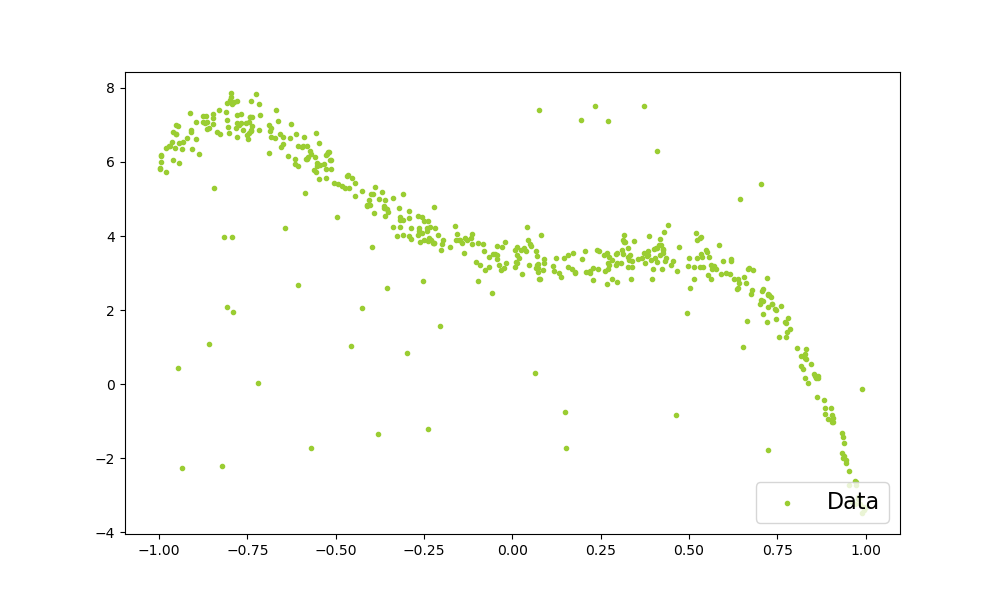
\includegraphics[width=0.95\columnwidth]{images/scatter_plot.png}
\caption{Polynomial function generated with random noise.}
\label{fig:polynomial_data}
\end{figure}
  
\section{Methods}

The original dataset consists of 500 data points, which were split into training (81\%), 
validation (9\%), and test (10\%) sets. No outlier removal was performed. 
All models were trained using the training set, evaluated with the validation set for model selection, 
and finally evaluated on the test set after model selection. The evaluation process involved three key steps: 
initial screening with validation, cross-validation of selected models, and final evaluation on the test set.

\subsection{Initial Screening with Validation}
Various models, including k-NN, linear regression variants, and polynomial regression with regularization, were first evaluated using a validation set. 
The purpose of this step was to quickly assess model performance and identify promising candidates.

\subsection{Cross-Validation of Selected Models}
Based on the validation results, a subset of models was chosen for cross-validation. Cross-validation was used to provide a more robust evaluation with
\( k = 10 \) folds. The average performance across the folds was used to further narrow down the best-performing models.

\subsection{Final Testing on Test Set}
After cross-validation, the best models were evaluated on the test set to determine their generalization performance.

\subsection{Models}

We tested several different models, including k-Nearest Neighbors (k-NN), 
various linear regression models(Huber and RANSAC), and polynomial regression with regularization (Ridge and Lasso).

\subsubsection{k-Nearest Neighbors (k-NN)}
The k-NN algorithm was tested with CAMBIAR Y AGREGAR GRIDSEARCH \( k = 1 \), \( k = 5 \), \( k = 10 \), \( k = 15 \), and \( k = 20 \). 
The optimal \( k \) value was chosen based on validation set performance.

\subsubsection{Linear Regression Variants}
Despite knowing that a linear model might not be the outmost appropiated for this task, 3 variants were implemented
to compare with other methods:

\begin{itemize}
    \item Standard Linear Regression.
    \item Huber Regression.
    \item RANSAC Regression.
\end{itemize}

\subsubsection{Polynomial Regression with Regularization}
Polynomial regression models were fitted with degrees ranging from 2 to 12. Additionally, 
Lasso and Ridge regression were applied with a regularization parameter \( \lambda = 0.01 \), 
obtained from a grid search over \( \{0.01, 0.1, 1, 10, 100\} \). 

\subsection{Evaluation Metrics}
The models were evaluated using two primary metrics:
\begin{itemize}
    \item Mean Squared Error (MSE).
    \item \( R^2 \) Score.
\end{itemize}


\section{Results}

The following steps were taken to assess model performance:

\subsection{Initial Validation Results}
The first screening of models was done using the validation set. Table \ref{tab:validation} shows the MSE and \( R^2 \) 
scores for the various models during the validation phase. Based on these results, several models were selected 
for cross-validation.

\begin{table}
\centering
\caption{Initial validation performance}
\label{tab:validation}
\begin{tabular}{|l|l|c|c|}
\toprule
                           Model &   MSE &    R2 \\
\midrule
                      KNN (k=17) & 0.514 & 0.916 \\
                          Linear & 0.978 & 0.841 \\
                           Huber & 1.059 & 0.828 \\
                          RANSAC & 1.337 & 0.782 \\
           Polynomial (degree=6) & 0.425 & 0.931 \\
Ridge (degree=6, $\lambda=0.01$) & 0.430 & 0.930 \\
Lasso (degree=6, $\lambda=0.01$) & 0.474 & 0.923 \\
           Polynomial (degree=7) & 0.509 & 0.917 \\
Ridge (degree=7, $\lambda=0.01$) & 0.465 & 0.924 \\
Lasso (degree=7, $\lambda=0.01$) & 0.474 & 0.923 \\
\bottomrule
\end{tabular}
\end{table}


\subsection{Cross-Validation Results}
The selected models (k-NN with \(k=15\) CAMBIAR 15, polynomial regression with degree 6, and Ridge regression with degree 6 and \(\lambda = 0.01\)) were then evaluated using cross-validation. 
The cross-validation results are summarized in Table \ref{tab:cross_validation}. 
Cross-validation confirmed that k-NN and polynomial regression were the best candidates.

\begin{table}
\centering
\caption{Cross-validation performance}
\label{tab:cross_validation}
\begin{tabular}{|l|l|c|c|}
\toprule
                           Model &   MSE &    R2 \\
\midrule
           Polynomial (degree=6) & 1.770 & 0.682 \\
Ridge (degree=6, $\lambda=0.01$) & 1.769 & 0.682 \\
Lasso (degree=6, $\lambda=0.01$) & 1.813 & 0.676 \\
           Polynomial (degree=7) & 1.763 & 0.684 \\
Ridge (degree=7, $\lambda=0.01$) & 1.765 & 0.683 \\
Lasso (degree=7, $\lambda=0.01$) & 1.813 & 0.676 \\
                      KNN (k=17) & 1.803 & 0.705 \\
\bottomrule
\end{tabular}
\end{table}


\subsection{Test Set Results}
Finally, the selected models were tested on the test set. Table \ref{tab:tests} shows the final MSE and \( R^2 \) scores on the test set 
for the top-performing models. k-NN with \(k=15\) CAMBIAR ESTE 15 provided the best generalization, 
slightly outperforming polynomial regression with degree 6.

\begin{table}
\centering
\caption{Tests}
\label{tab:tests}
\begin{tabular}{|l|l|c|c|}
\toprule
                           Model &   MSE &    R2 \\
\midrule
                      KNN (k=17) & 1.127 & 0.807 \\
           Polynomial (degree=6) & 1.146 & 0.803 \\
Ridge (degree=6, $\lambda=0.01$) & 1.143 & 0.804 \\
\bottomrule
\end{tabular}
\end{table}


\section{Discussion}


\section{conclusion}

\end{document}
